\subsection{Bitcoin}
% 
Created in 2009, Bitcoin is the first ever digital currency, that operates without a central authority in a completely decentralised manner. It is a cryptocurrency with largest market capitalisation\footnotemark and probably the most famous cryptocurrency worldwide.
% 
\footnotetext{Over USD 115 billion as of 01-04-2018. \url{https://coinmarketcap.com/}, accessed 01-04-2018
}
% 
Bitcoin was proposed by person or group under a pseudonym Satoshi Nakamoto, whose identity is not known to date \cite{Feins2017SatoshiBitcoin}. The initial proposal consisted of a white-paper describing the system \cite{NakamotoBitcoin:System} and the first implementation written in  C++ \footnotemark.
% 
\footnotetext{Original repository has been moved from SourceForge and can now be found on Github. \url{https://github.com/bitcoin/bitcoin/tree/4405b78d6059e536c36974088a8ed4d9f0f29898}, accessed 01-04-2018}

In the white-paper, Nakamoto proposes a decentralised currency, based on a proof-of-work blockchain. The blockchain is made up of blocks, where each block comprises a different set of transactions \cite{Decker2013InformationNetwork, Judmayer2017BlocksMechanisms}.

\paragraph{Proof of work}
To include a new block in the blockchain, certain amount of work needs to be carried out by the node. This is a protection against the attempts to include counterfeit data in the blockchain. As discussed earlier, to falsify a past block, an attacker would need to recalculate all the subsequent blocks. Furthermore, they would need to provide proof-of-work for all the subsequent blocks. Since the proof-of-work is computationally intensive, it would be practically impossible for the attacker to outpace the honest nodes.

In case of Bitcoin, the proof-of-work consist of finding such a hash value, that is below a given constant -- \textit{target}. In Bitcoin, this hash value is computed over the hash value of previous block, timestamp\footnotemark, root hash of transactions and random number, called \textit{nonce}. The work of the nodes consists of generating a new nonce and computing a new hash. If value of this hash is smaller than the target, a valid block is produced and can be broadcasted to other nodes. Figure \ref{fig:blocks-bitcoin} shows the composition of the block in detail. By design, a new block should be mined approximately every 10 minutes. The network automatically adjusts the value of the target to meet this requirement (if the value of the target remained the same, increasing speed of computers would result in faster block production speed) \cite{Decker2013InformationNetwork}.
% 
\footnotetext{The timestamp is a local UNIX time of the node. However, this timestamp does not to be very accurate (approximate allowed accuracy is $\pm$ 1 hour). It can happen, that the timestamps in blocks are not in order. The goal of the timestamp is to increase the difficulty of forging the blocks. \url{https://en.bitcoin.it/wiki/Block_timestamp}, accessed 01-04-2018}
% 
\begin{figure}[ht]
    \centering
    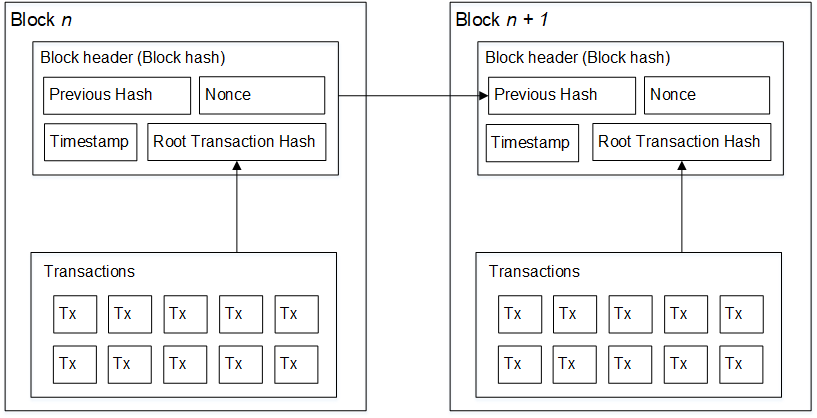
\includegraphics[width=.95\textwidth]{blocks-bitcoin}
    \caption{Composition of Bitcoin blockchain. \textit{Work} consists of repeatedly hashing the block header, trying different nonce every time.}
    \label{fig:blocks-bitcoin}
\end{figure}
% 
\paragraph{Network of nodes}
Each node carries out work at its own pace, trying different values for nonce and hashing the block header. This process is also referred to as \textit{mining}. Once the hash is below the current threshold, a new block is mined. The new block is then broadcasted to all the nodes connected to the network \cite{NakamotoBitcoin:System}. When a node receives a block it has not seen before, it first verifies the transactions in the block and then introduces it to its peers. The average time for a block to reach the whole network is 12.6 seconds \cite{Decker2013InformationNetwork}. It is well below the block generation speed (1 block approximately every 10 minutes), however, it is not crucial for the network that every node has the latest block. ``\textit{If a node does not receive a block, it will request it when it receives the next block and realises it missed one.}'' \cite{NakamotoBitcoin:System}.
% 
\paragraph{Transactions}
A Bitcoin transaction is the act of moving the funds from one account to another. An account is pair of a public and private key. Bitcoin uses \acrfull{ecdsa} for the key pair generation \cite{Decker2013InformationNetwork}. The account is identified by its public address. Public address is generated from the public key 

% Add a figure explaining the address generation process.

% Write about merkle trees and the root hash


\paragraph{Value}
Besides the system described above, Bitcoin also referrers to a basic \textit{unit} of the currency. Bitcoin is further divisible into smaller units. Smallest unit is 1 satoshi. 1 Bitcoin contains 100 000 000 satoshi. 1 Bitcoin at the time of writing has a value of EUR 5 666. The value of Bitcoin is very volatile and has increased and decreased by tens or percents, sometimes even within hours \cite{Adkisson2018WhyVolatile}. The peak in the value of Bitcoin has occured on December 16, 2017 when 1 Bitcoin was traded for around EUR 16 500.

\subsubsection{Alt-coins}

% Maybe mention slightly